\chapter{General Project Context}
\label{chap:General Project Context}

% "*" makes the section unnumbered

\section*{Introduction}

Use this template as you wish, change what you want to change, the section titles are only examples, you don't have to follow them to the letter.


This is an example of me citing the 1st reference in the bibliography at the end of this report \cite{ref1}. Use it well!

The next section contains the README text that's also found in the left part along with the other files.


\newpage

\section{READ\_ME}

Hi! 

This template is a combination of multiple student and teacher PFE report templates that I have compiled into one that hopefully will satisfy your needs.
\\

It is in English, but I have included the french "Page de garde" if you want to use it, and the rest of the paper is easily translatable.
\\

This document is compiled using pdfLatex Compiler, so make sure you select it in the menu on the top left of the page. You can change the font size there along with other things.
\\

Some table, figure, list or formatting codes can be found in the "Codes\_needed.tex" file in this same folder, use them well.
\\

The organisation of this template is as follows: 
\\
The main compilation file is main.tex, any file you want to add, should be added there using, %\chapter{General Project Context}
\label{chap:General Project Context}

% "*" makes the section unnumbered

\section{Introduction}

This chapter aims to conduct an initial exploration of the project, in order to better understand the system requirements, and to position the project within its organizational and contextual environment. It provides an overview of the hosting organization Orange Business Morocco, then reveals the general theme of the project by introducing its intentions and specifications, followed by the various approaches applied, including the recommended methodology for project management and the resulting planning.


\newpage


\section{Presentation of host organization}



\subsection{Company Overview}

\begin{figure}[H] 
    \centering
    
\includegraphics[width=7cm]{Logos/ob.png}
    \caption{OBS logo}
    %\label{fig:my_label} %Optional (If you want to reference the figure in later chapters)
\end{figure}

In 2000, following the opening of the telecommunications market to competition in Europe, France Télécom, the historic French operator, acquired the British brand Orange. At the same time, the Senegalese group Sonatel was created in the late 1980s, resulting from the merger of the Office des Postes et Télécommunications and TéléSenegal. Sonatel was privatized in 1997 and integrated into France Télécom's capital.

In France, France Télécom, quickly becoming a leader thanks to the quality of its networks, gradually unified all the group's subsidiaries under the name Orange. By 2009, Orange had a presence in more than 30 countries and served over 123 million customers.

On July 1, 2013, following a vote at a general meeting, France Télécom officially changed its name to Orange. This transformation marked a new chapter for the company while retaining a cultural heritage inherited from the public service. France Télécom's historic installations played an important role in the French telephone network, paving the way for the rise of mobile telephony and the beginning of a new revolution: the Internet.

Orange operates in several regions, notably in Europe, Africa, and the Caribbean. In 2019, it was considered the leader or second operator in 75% of the European countries where it is present, and in 83% of the countries in Africa and the Middle East. Orange offers telecommunications equipment and services for individuals, professionals, and businesses.

Orange Business operates in 166 countries and serves its customers in 220 countries and territories (Table 1.1).
\begin{longtable}[c]{| m{4.4cm} | m{11cm} |}
          \hline
          Date of Establishment & 2006 \\
          \hline
          Legal Form & Legal Form \\
          \hline
          Management & Christel Heydemann (CEO, Orange S.A)
          Helmut Reisinger (CEO, Orange Business Services) \\
          \hline
          Headquarters & Paris, France \\
          \hline
          Parent Company & Orange \\
          \hline
          Activity & Telecommunications
          Information Technology Services \\
          \hline
          Subsidiaries & Orange Application for Business, Business et Decision \\
          \hline
          Website & \url{http://www.orange-business.com} \\
          \hline
          \caption{Orange Business Information}\\
\end{longtable}

\subsection{Orange Business Morocco}
Orange Business Morocco is a newly established entity in 2018 in Rabat, specializing in the design and development of application services and system integration in various domains. It works on behalf of various expertise of Orange Business Services. Several companies have provided application services for Orange Business Services, such as Almerys, a health third-party payer operator. OBS IT Morocco is founded to take control of its applications, optimize and rationalize costs, bring development teams closer to business directions, and improve IT solution delivery times for TTM. By following an Agile way of working to deliver functionalities regularly that create the most value and adopting a simple and automated development and production environment to focus on the essentials. OBS IT Morocco uses the cloud, DevSecOps tools, and automated testing and feedback utilization to enrich applications while ensuring a user-centered approach. By guaranteeing versatile, autonomous, and committed teams to manage all activities on their applications (collecting requirements, drafting user stories, development, testing, integration, deployment, support).

\subsection{Organization and Organizational Chart}
OBS Morocco, overseen by a director Mrs. Rym Sahnoun who is the highest authority, is organized into operational poles whose goal is to focus its energies on a daily basis towards customer satisfaction. Teams are organized by Orange business services. I completed my internship in the OBS IT entity managed by Mr. Aarab Abderrahim and specifically Customer Marketing Innovation (Fig. 1.6) in the DevSecOps/TAAS team attached to Mr. Moustachi Mouhcine, IT RUN Manager (see Fig. 1.7).

\begin{figure}[H]
  \centering
  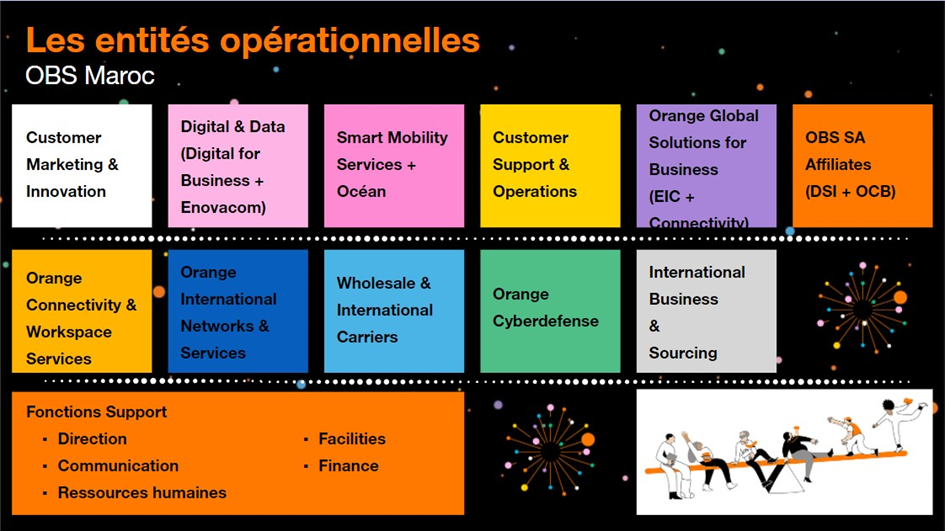
\includegraphics[width=17.5cm]{Figures/entite.png}
  \caption{OBS IT Morocco's operating entities}
  \label{fig:vue-snoc-pos}
\end{figure}

\textbf{CMI}: This is the IT Department of the Orange Group. Its goal is to create efficient software development, entity-oriented, based on the best practices of a software factory (digital factory model). This entity adopts an agile delivery model, possesses a simple and automated development and production environment. It is a versatile, autonomous, and committed team to manage all activities related to the applications entrusted to it: from collecting customer needs and requirements, to writing user stories, through development, testing, and integration, before reaching deployment and support.

\begin{itemize}
  \item Enrich the relationship between companies and their customers through a digital approach and a 360° customer journey.
  \item Exploit machines and communicating objects that transmit real-time data to create new sources of revenue and differentiation.
  \item Make use of the data produced by companies and their customers to innovate and personalize their products and services.
  \end{itemize}
  
\textbf{OCWS}: This entity is composed of 3 poles with different missions. The first center, internationally / in Morocco, manages the operational part. A pre-sales team provides technical assistance to commercial engineers to help them negotiate contracts. A BUILD team's missions include deploying network solutions for customers and offering them the best possible connectivity experience through various technologies such as SDWAN, WIFI, LAN, etc.

\vspace{10pt} 

\textbf{OCD}: This is the entity that designs cybersecurity services that support customers in the Maghreb and West Africa, throughout the life cycle of threats that can impact client companies. They have 5 main missions:
  
  \begin{itemize}
  \item Anticipate the latest threats.
  \item Identify the assets and critical data of customers, prepare the security strategy, and ensure its proper functioning.
  \item Deploy appropriate technology to defend the organization and manage it continuously.
  \item Monitor, qualify, and analyze security alerts to confirm if there has been an incident.
  \item Qualify, contain, and remedy attacks. Thanks to their sectoral expertise, they can offer tailor-made services to meet customer challenges.
  \end{itemize}
  
  \textbf{Orange Connectivity}: Entity responsible for marketing OBS Connectivity data offers (Internet, Ethernet, VPN).
  
  \vspace{10pt} 

  \textbf{Missions in Morocco}: Management of pricing for offers marketed in France and internationally (definition and update of standard prices, calculation of custom prices).
  
  \vspace{10pt} 

  \textbf{OINIS}: Orange International Networks Infrastructures \& Services' mission is to design, deploy, and operate reliable, secure, and high-quality international network infrastructures and services for businesses, wholesale customers (operators), and subsidiaries.

  \vspace{10pt} 

  \textbf{WIN IC}: This is the commercial arm of OINIS. This entity provides international connectivity services to operators and internet service providers worldwide.

  \vspace{10pt} 
  
  \textbf{The Business Unit EIC} (Enriched Interactions and Collaboration): Straddling digital \& data and connectivity, its goal is to design and bring to market communication and collaboration offerings from Orange Business Services: voice solutions, conference solutions, unified communications suites, and contact center solutions.

\section{Project presentation}
\subsection{General project context}
In today's world, ensuring the sustainability of IT practices is paramount. When it comes to IT professionals, it is imperative to prioritize eco-friendly strategies from the outset of the development process.

As a developer, you may not be required to master the intricacies of environmental impact assessments, as there are several reliable tools available to assess the carbon footprint of IT solutions. By integrating these assessments into the CI/CD pipeline and implementing effective remediation strategies, organizations can significantly reduce the environmental cost associated with IT operations.

This includes not only the direct costs of energy consumption but also the broader environmental impact of resource depletion and pollution. Consequently, IT teams have embraced a new approach known as Green IT, which promotes the integration of sustainability principles into IT practices and encourages close collaboration between environmental experts, developers, and IT engineers.

This approach ensures that environmental considerations are addressed at every stage of the development and delivery process, thereby fostering a more sustainable IT ecosystem.

The project is set within this broader context of optimizing Green IT practices at Orange Business Services Morocco. To support this initiative, the DevSecOps team has been recently created within the IT RUN entity to fulfill two main missions:

\begin{itemize}
    \item \textbf{Cloud DevSecOps}: Design, build, and implement Cloud services and DevSecOps tools.
    \item \textbf{REaCT}: Implement the DevOps mindset within the company and support development projects.
\end{itemize}

\begin{figure}[H]
  \centering
  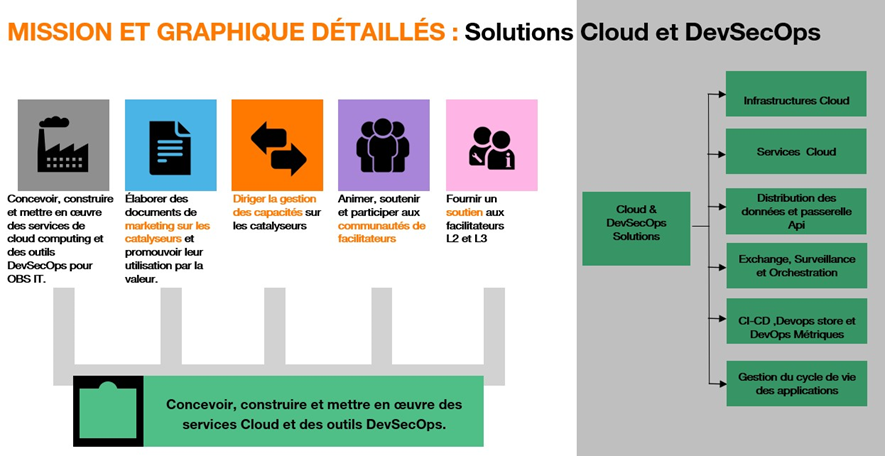
\includegraphics[width=17.5cm]{Figures/mission.png}
  \caption{Cloud \& DevSecOps missions}
\end{figure}
\subsection{Problematic}

While Orange Business Services Morocco has established efficient CI/CD pipelines using GitLab, there is a lack of focus on environmental sustainability and energy efficiency within their DevOps processes. The current approach prioritizes swift software delivery but overlooks the environmental impact of development and deployment activities. This neglect of Green IT principles hinders efforts to reduce energy consumption and carbon emissions associated with the organization's IT infrastructure, particularly its Kubernetes clusters. The challenge lies in integrating Green IT considerations seamlessly into existing DevOps workflows without compromising efficiency or productivity. Thus, the problematic revolves around balancing the need for rapid software delivery with environmental responsibility, requiring the development of strategies and tools to monitor and optimize energy usage and carbon footprint throughout the CI/CD pipeline
\section{Project planning and management}
\subsection{Adopted methodology}

To ensure optimal progress of our project, we have chosen to use the agile Scrum method (illustrated in Fig. 1.10).

\begin{figure}[H]
  \centering
  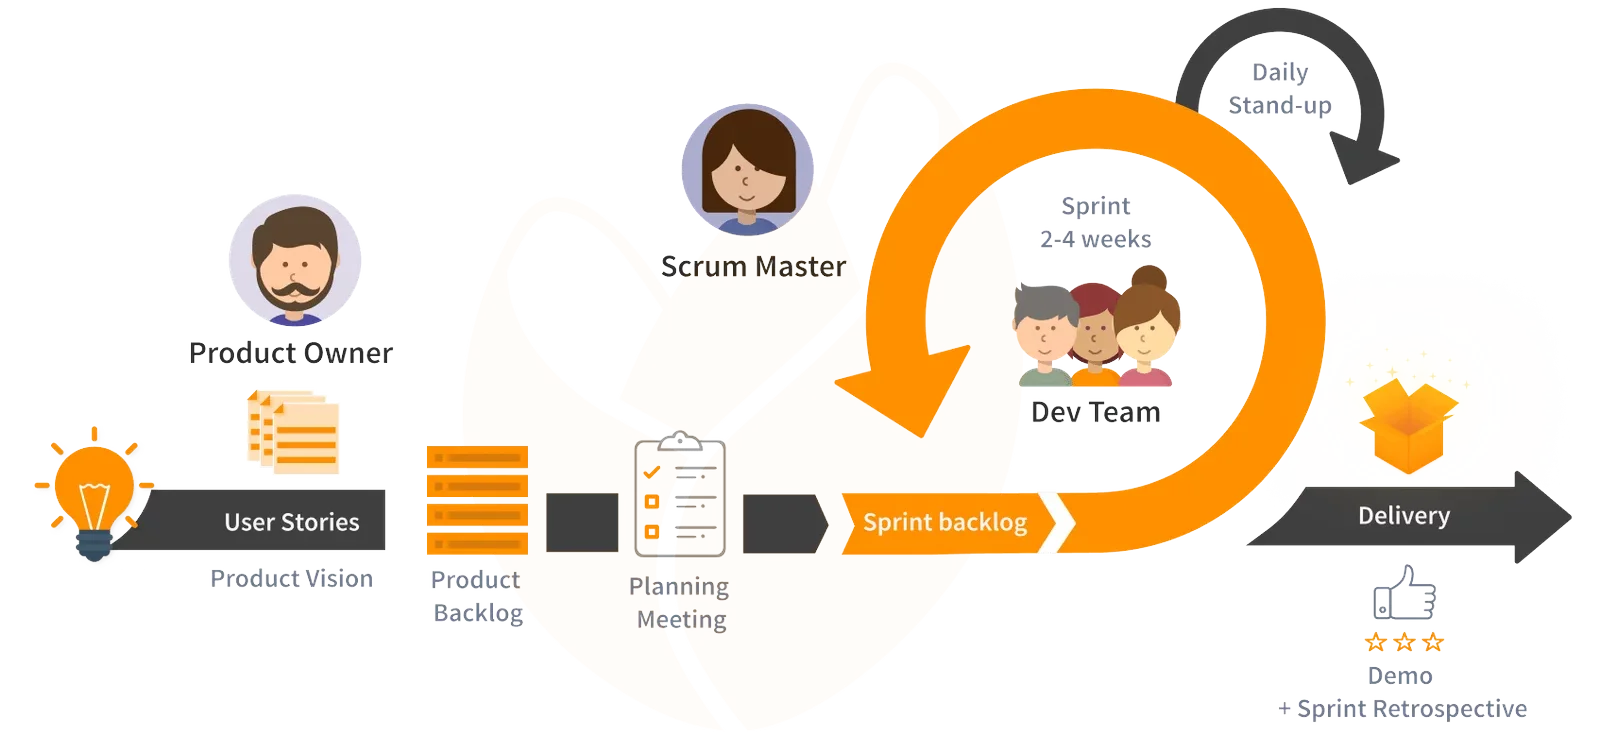
\includegraphics[width=17.5cm]{Figures/scrum.png}
  \caption{Scrum methodology}
\end{figure}

This approach will enable us to best meet the needs of the company while minimizing the risk of delays and ensuring the satisfaction of all stakeholders.

Scrum is an agile project management method that was first introduced in an article by Hirotaka Takeuchi and Ikujiro Nonaka in 1986, published in the Harvard Business Review under the title "The New Product Development Game". It was developed in the 1990s and formalized by Ken Schwaber and Jeff Sutherland in 1995.

The fundamental principle of this method is to iteratively focus on the features to be implemented. The project is divided into functional modules that are developed, tested, and delivered in iterative sequences called "sprints". Each sprint aims to achieve a specific goal, from which the features to be implemented are chosen.

We have adapted the Scrum method to our project by dividing it into sprints of two to three weeks. At the end of each sprint, a meeting is organized with the Scrum Master and the Product Owner to review the work done during the period and set the tasks and objectives for the next sprint. If differences are noted during the inspection, we adapt the process in question. To do this, we have set up weekly meetings led by the Scrum Master, during which each team member presents the status of their tasks, reports any encountered blockers, and outlines the actions to be taken for the next period as well as future prospects. This approach has allowed us to clearly define the objectives for each increment and adapt them as needed, while also allowing us to complete or modify the list of features to be implemented for the upcoming sprints.

\subsection{Project Planning}
Planning is an essential step in project management, as it allows defining the tasks to be performed, setting objectives, coordinating actions, mastering resources, reducing risks, monitoring ongoing actions, and reporting on the project's progress. In our case, we began by breaking down the project into tasks, then proceeded with a risk assessment before establishing a Gantt chart to have an overview of the project's progress.

\subsection{Project Breakdown into Sprints}

The project is divided into sprints, with each sprint being a crucial step in the project's completion.

\begin{figure}[H]
    \centering
    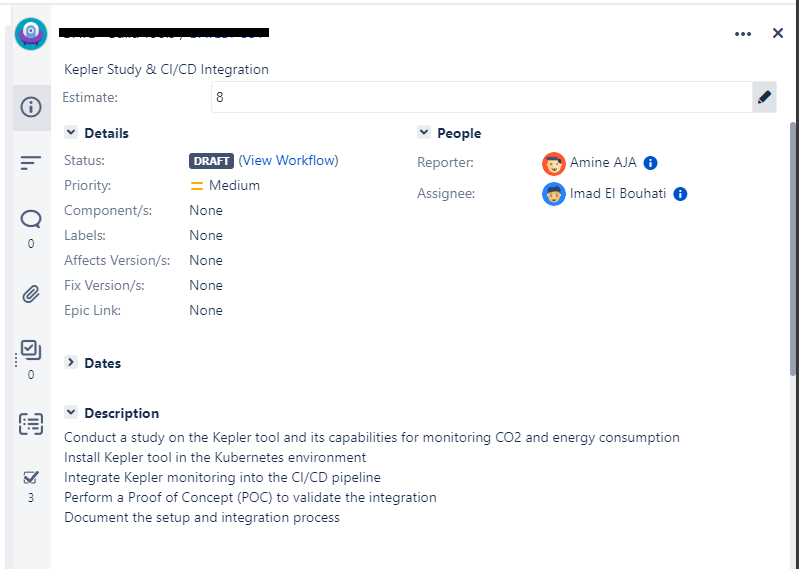
\includegraphics[width=16cm]{Figures/us-1.png}
    \caption{Tasks performed}
\end{figure}

\begin{figure}[H]
  \centering
  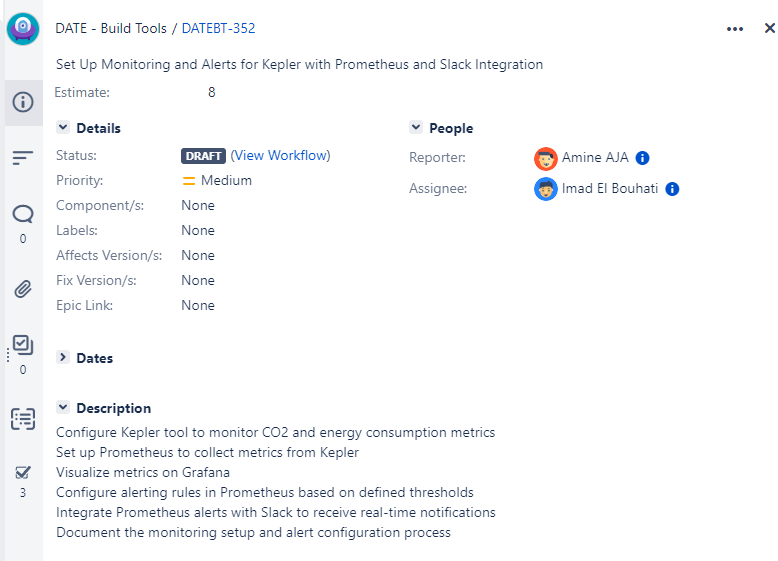
\includegraphics[width=16cm]{Figures/us-2.png}
  \caption{Tasks performed}
\end{figure}

\subsection{Communication Tools}

In the dynamic environment of modern project management, effective communication is paramount to ensure seamless collaboration and timely decision-making. Utilizing robust communication tools can streamline interactions within teams and enhance overall productivity.

\begin{figure}[H]
  \centering
  
\includegraphics[width=3cm]{Logos/microsoft_teams_logo.png}
  \caption{Microsoft Teams Logo}
\end{figure}

Microsoft Teams serves as a cornerstone for communication within our DevSecOps team. This platform offers a comprehensive suite of features, including instant messaging, video conferencing, file sharing, and integration with various productivity tools. Team members can collaborate in real-time, hold meetings, and access project-related resources, fostering efficient communication and collaboration.

\subsection{Internship Progress}

The Gantt chart is a visual presentation method that allows positioning in time the different stages, activities, tasks, and resources involved in a project. Tasks are listed on the rows, while the columns represent days, weeks, or months. The bars symbolizing each task have a length proportional to the expected duration.
\begin{figure}[H]
    \centering
    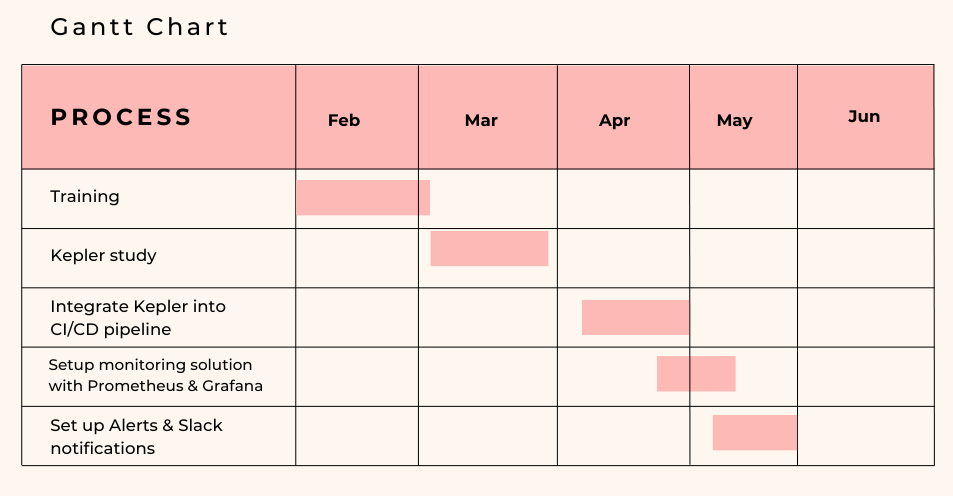
\includegraphics[width=16cm]{Figures/gantt-chart.png}
    \caption{Gantt Chart}
\end{figure}
\section{Conclusion}
In this chapter, we first introduced Orange Business Morocco, the organization involved in the project. Then, we established the general framework of the project before presenting the specific problem to be addressed. We also explained the working method we adopted and provided an overview of the schedule that was followed throughout the project. In the next chapter, we will move on to the functional and non-functional analysis of our project, as well as detailed design. This phase will define the specifications necessary for the development of the overall project architecture. for example. 

Remember to change the PDF Title and author name before the begin document command.
\\

Packages.tex is where you import packages and could modify their options.
\\

The frontmatter folder contains unnumbered chapters that come before the actual chapters, so the resumes and acknowledgments are there. The pages are numbered in Roman numbers.
\\

The chapters folder obviously contains the main chapters of the report, usually the first one is an intro, of both the project and the company, the last one is a conclusion chapter, I made it unnumbered here but you do you.
\\

The endmatter folder contains the appendices, acronyms, glossary, and Complementary figures, tables and codes. Consider checking this link \url{https://libguides.usc.edu/writingguide/appendices} for more info. Usually you add an appendix for each subject you'll talk about it, each with its own codes, tables, figures and text.
\\

The bibliography can be found at the end of main.tex file.
\\

And to organise your figures better, upload the logos to the logos folder, and content related figures should go in the figures folder, where you can add sub folders.
\\

Along the template, make sure to read my comments, they can be helpful to understand the purpose of a command or option. 
\\

When you finish writing your thesis, make sure to verify that you didn't leave any generic line or link. Revise it well.
\\

There are 10 warnings that show up in this template, some I couldn't manage to solve (or understand), and some I left since they are necessary for what I intend of this template.
\\

Obviously this template is only a suggestion, it is not perfect in any sense, you can improve it in the way that suits you, so search away, and get used to reading the documentation.
\\

Also consult with your supervisor, as each teacher has their own opinion on what constitutes the ideal report.
\\

Finally, I hope you have enjoyed your time at INPT as much as I did, and Good Luck :D
\\

-Mery


\subsection{Codes\_Needed}

This subsection includes codes for different elements you will need: figures, tables, lists...

Copy the codes you want and test them in the chapter files.

if you want symbols and other text styles, visit this link: 

\href{https://www.cmor-faculty.rice.edu/~heinken/latex/symbols.pdf}{Symbols}

Read the comments !!

% Content division

%\chapter{Comes first}, then \section{}, then \subsection{}, then \subsubsection{}.

\subsubsection{Text formatting}

\textbf{This text is bold}

\textit{This text is italic}

\underline{This text is underlined.}

\st{This text is struck out.}

\textsc{This text is capitalized.}

%Use \paragraph{To start a paragraph}


Some characters like "\%", "\$" and "\&" are significant in Latex code, so to include them in normal text, use the backslash character before them.
To print out backslash, use \symbol{92}


Documentation: \href{https://www.overleaf.com/learn/latex/Bold%2C_italics_and_underlining}{Italics and underlining}


\subsubsection{Figures} 

\begin{figure}[H] 
    \centering
    
\includegraphics[width=4cm]{Logos/Logo_INPT.png}
    \caption{Caption}
    \label{fig:my_label} %Optional (If you want to reference the figure in later chapters)
\end{figure}

%[width=7cm] you control the size of the image. other options include: 
%[height=7cm] or [scale=0.5] (means half the size of the original image)


Documentation: \href{https://www.overleaf.com/learn/latex/Inserting_Images}{Images}


\subsubsection{Tables} 

Simple table without borders:
\\

\begin{tabular}{ll}
  First & Second \\
  Third & Fourth
\end{tabular}
\\

More complex table with borders:
\\

\begin{tabular}{|l|c|r|} \hline
  Left aligned column & Centered column & Right aligned column \\ \hline
  Text & Text & Text \\ \hline
\end{tabular}
\\

Example of a short table

%{5cm} is the cell length, you can change it to suit your own table

\begin{table}[H]
    \centering
    \begin{tabular}{|m{5cm}|m{10cm}|}
        \hline
          Column1 & Column2 \\
        \hline
          Element11 & Element21 \\
        \hline
          Element12 & Element22 \\
        \hline
          Element13 & Element23 \\
        \hline
    \end{tabular}
    \caption{Table Example}
\end{table}


Example of a long table (that spans 2 pages or more), Latex will automatically split the table when it reaches the end of the page:

\begin{longtable}[c]{| m{4.4cm} | m{11cm} |}
\caption{Long table}\\
 \hline

 Cell & Description  \\ 
 \hline
 \endfirsthead

 \hline
 
 Cell & Description  \\ 
 \hline
 \endhead

        \hline
          Element11 & Element21 \\
        \hline
          Element12 & Element22 \\
        \hline
          Element13 & Element23 \\
        \hline
          Element14 & Element24 \\
        \hline
          Element15 & Element25 \\
        \hline
          Element16 & Element26 \\
        \hline
          Element17 & Element27 \\
        \hline
          Element18 & Element28 \\
        \hline
          Element19 & Element29 \\
        \hline
          Element110 & Element210 \\
        \hline
          Element111 & Element211 \\
        \hline
          Element112 & Element212 \\
        \hline
          Element113 & Element213 \\
        \hline
          Element114 & Element214 \\
        \hline

 \end{longtable}


Documentation: \href{https://www.overleaf.com/learn/latex/Tables}{Tables}


\subsubsection{Lists}

To start an unnumbered list, use:

\begin{itemize}
    \item 
    \item 
    \item 
\end{itemize}

To start a numbered list, use:

\begin{enumerate}
    \item 
    \item 
    \item 
\end{enumerate}



Documentation: \href{https://www.overleaf.com/learn/latex/Lists}{Lists}


\subsubsection{Code scripts or terminal}

Say you have a script or terminal command you want to include, you use the following code:

    \lstset{style=mystyle} %this style is already defined in Packages.tex
    
    \begin{lstlisting}[language=bash, caption= Code caption]
    
    root@eve-ng:~# mkdir -p /opt/unetlab/addons/qemu/timos-20.10.R12

    \end{lstlisting}


Documentation: \href{https://www.overleaf.com/learn/latex/Code_listing}{Code Listing}

\subsubsection{Math}

Some math formulas for you, test them in your chapters:

These are inline formulas: $x$, $a_i^2 + b_i^2 \le a_{i+1}^2$. Afterwards...

These are centered formulas: $$x,$$ $$a_i^2 + b_i^2 \le a_{i+1}^2.$$ Afterwards...

Some complex formula: $$P(|S - E[S]| \ge t) \le 2 \exp \left( -\frac{2 t^2 n^2}{\sum_{i = 1}^n (b_i - a_i)^2} \right).$$

Also you can use the first link for math symbols and other useful stuff:

Documentation: \href{https://www.cmor-faculty.rice.edu/~heinken/latex/symbols.pdf}{Symbols file again}



\newpage


\section{Presentation of host organization}



\subsection{Company Overview}

\begin{figure}[H] 
    \centering
    
\includegraphics[width=7cm]{Logos/ob.png}
    \caption{Company logo}
    %\label{fig:my_label} %Optional (If you want to reference the figure in later chapters)
\end{figure}



\subsection{Organizational Chart}


\begin{figure}[H] 
    \centering
    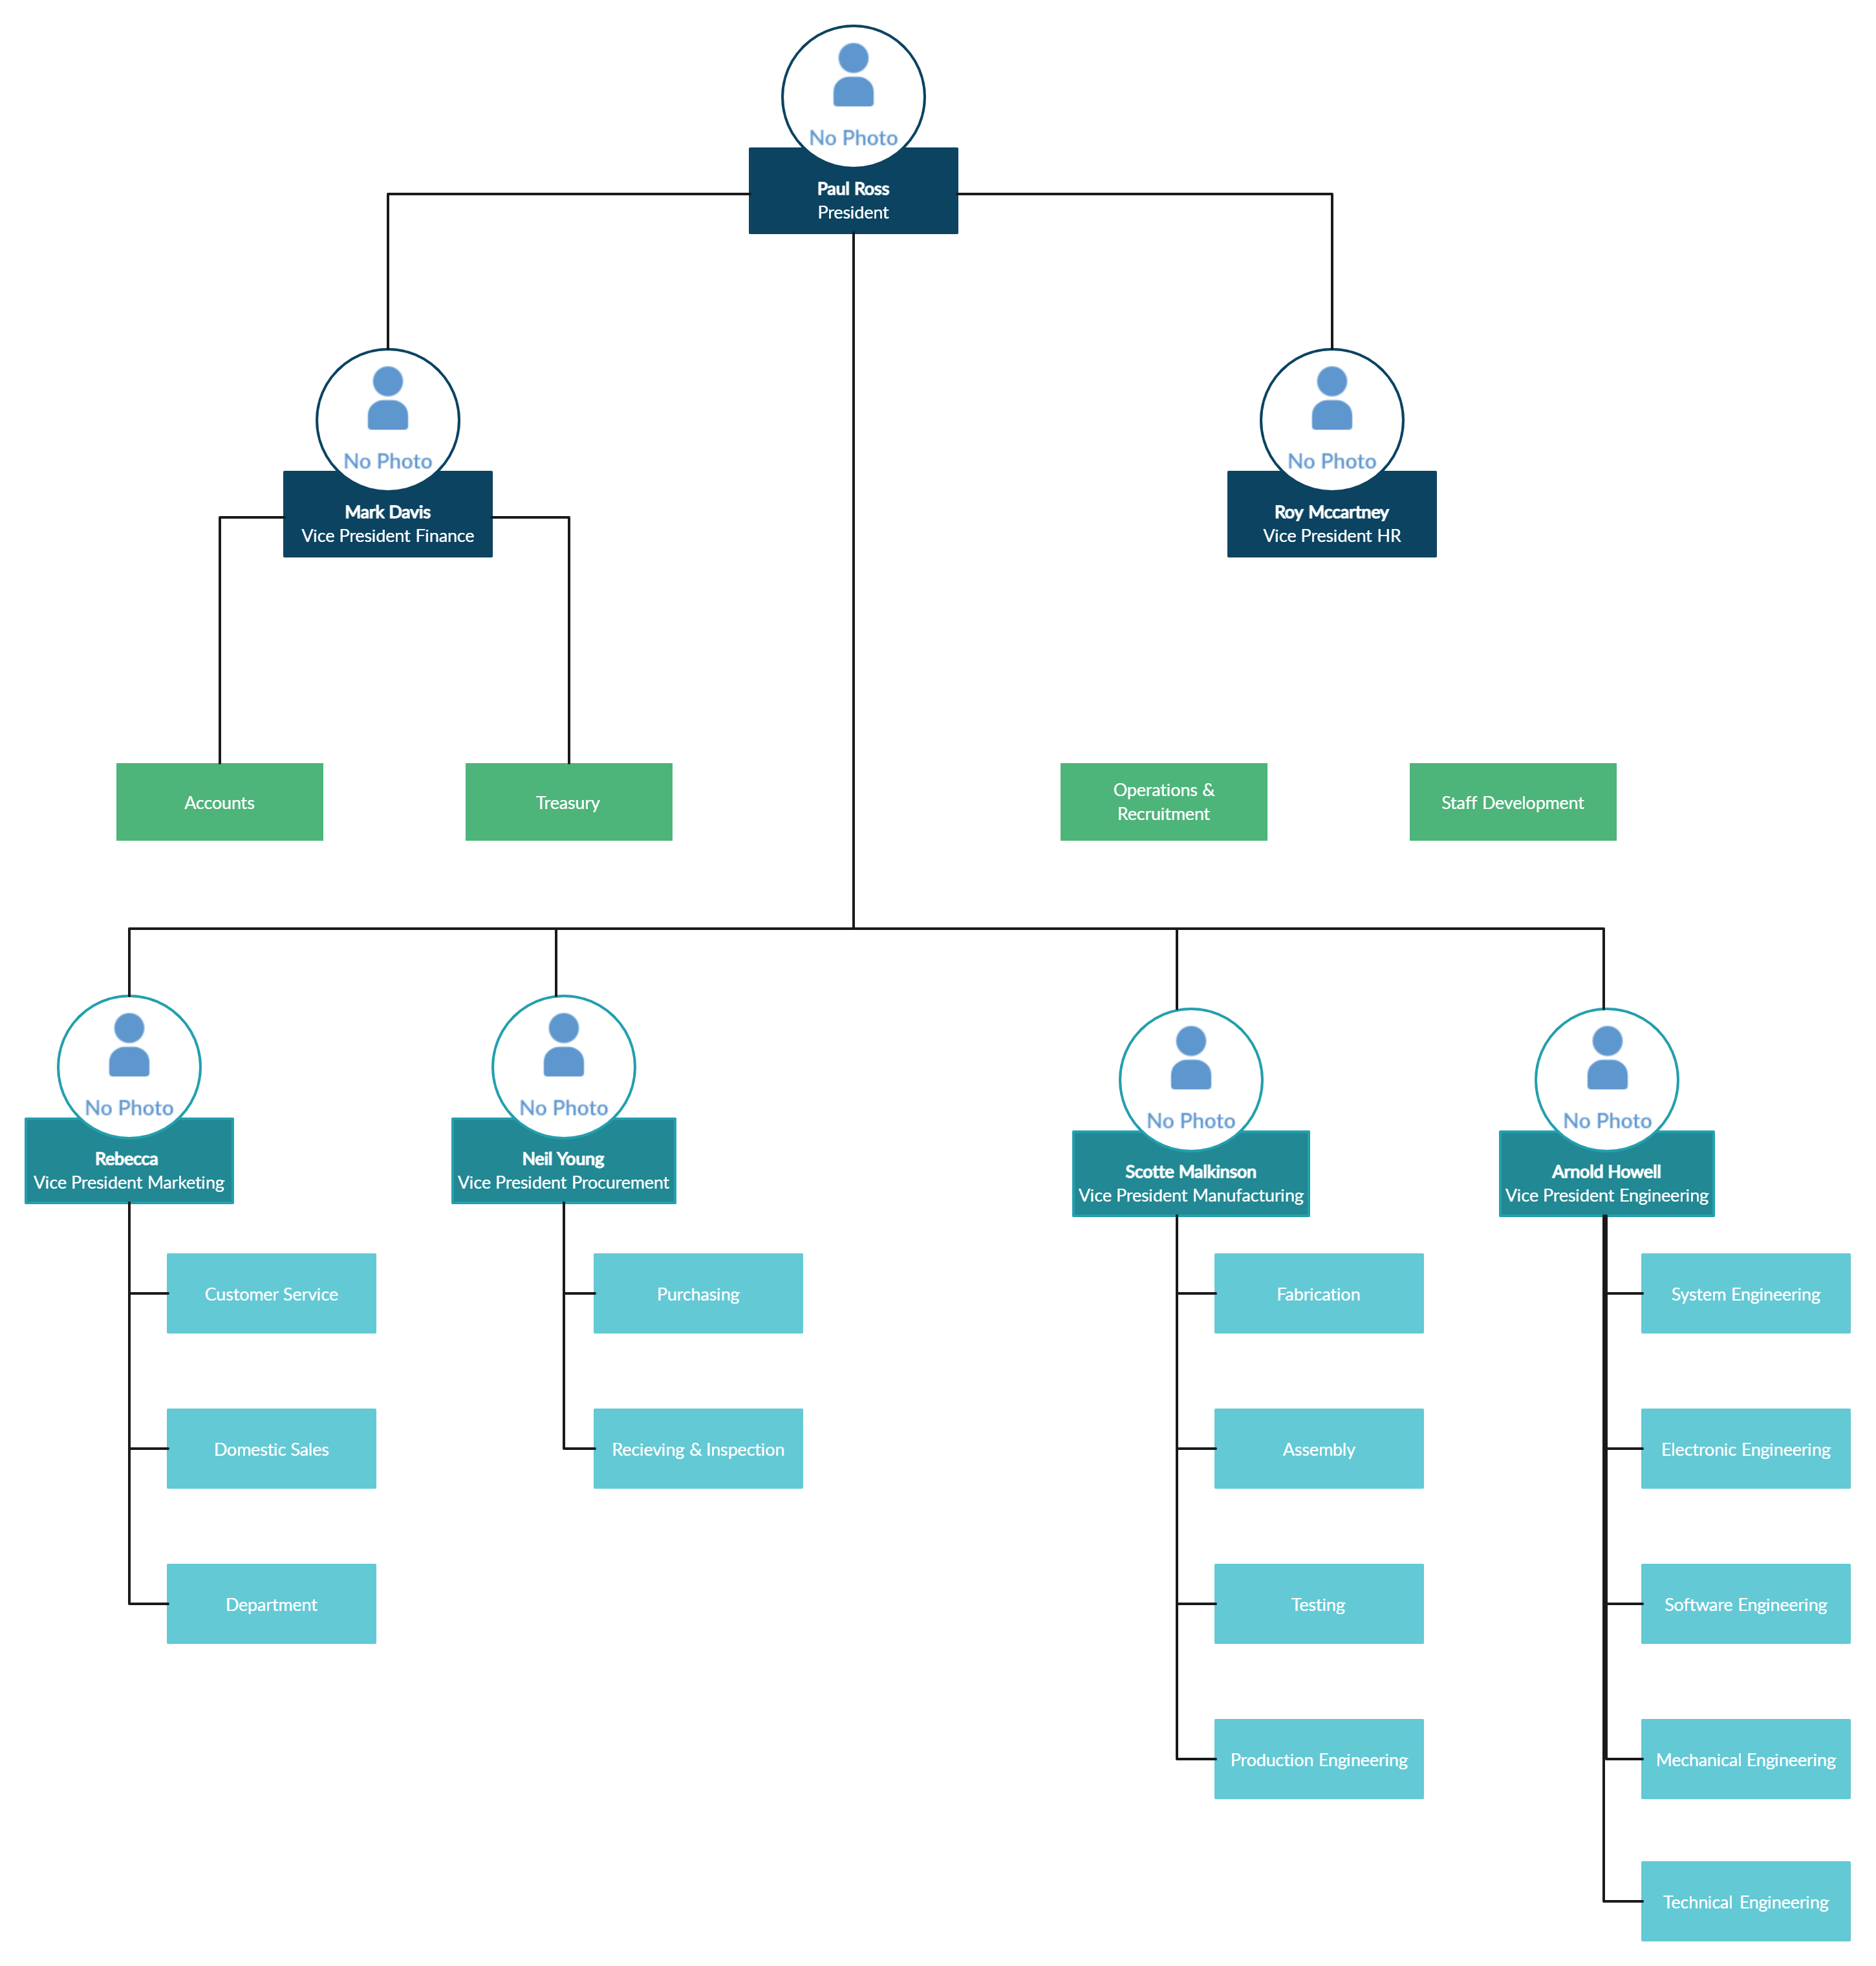
\includegraphics[width=12cm]{Figures/Organizational_Chart.png}
    \caption{Organizational Chart}
    %\label{fig:my_label} %Optional (If you want to reference the figure in later chapters)
\end{figure}










\section{Presentation of the project}


\subsection{Project Framework}



\subsection{Project objectives}





\subsection{Project Planning}

\begin{figure}[H] 
    \centering
    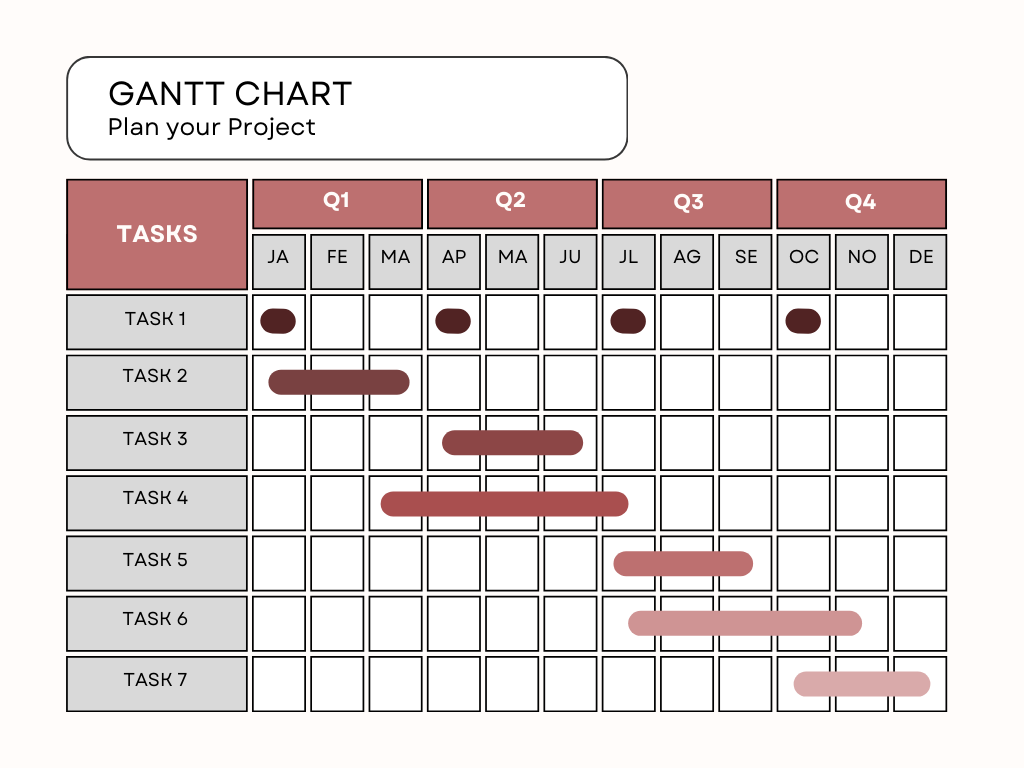
\includegraphics[width=12cm]{Figures/Gantt_Diagram.png}
    \caption{Gantt Diagram}
    %\label{fig:my_label} %Optional (If you want to reference the figure in later chapters)
\end{figure}

\newpage

\section*{Conclusion}

Lorem ipsum dolor sit amet, consectetur adipiscing elit. Praesent nec dapibus justo. Donec sagittis vulputate ante sed porttitor. Suspendisse sit amet nisl massa. Curabitur nec nisl condimentum, egestas ex vitae, dapibus enim. Etiam iaculis, erat faucibus pellentesque sagittis, nisi justo sollicitudin nibh, et condimentum augue massa non turpis. Proin commodo enim fermentum suscipit condimentum. Maecenas molestie, dui nec vestibulum rhoncus, arcu nisl faucibus neque, a ornare nisi massa ac eros. Aenean id velit sit amet lacus mattis varius. Donec fringilla massa sed nisi eleifend, a aliquet mi tempus. Nunc posuere euismod est, nec tristique augue lobortis non. Sed sodales sem ut metus tempus ullamcorper.
